\documentclass[11pt]{wbzine}
%packages
\usepackage{lipsum}
\usepackage[utf8]{inputenc}
\usepackage[T1]{fontenc}
\usepackage[ngerman]{babel}
\usepackage{coelacanth}
\usepackage{pdfpages}

\begin{document}

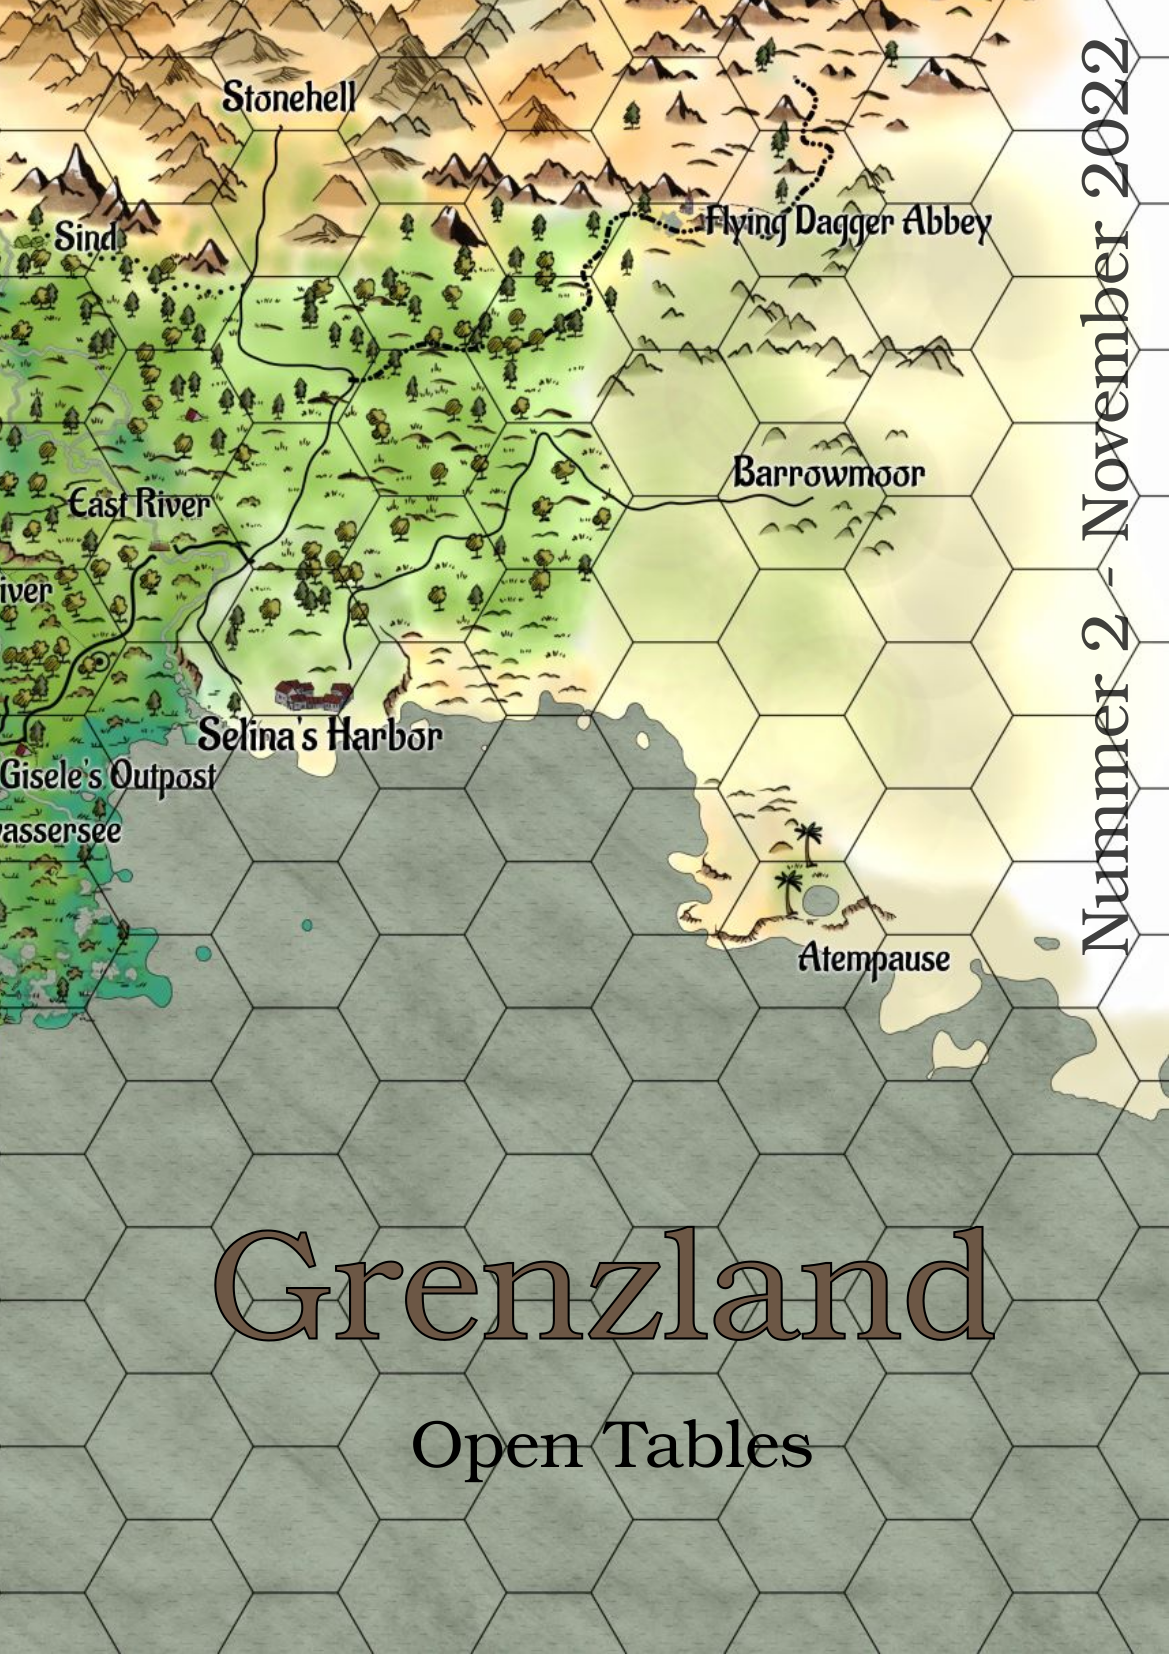
\includepdf{Frontcover.pdf}

\shipout\null
\addtocounter{page}{-1}

{\bfseries\fontsize{70}{55}
 \selectfont Grenzland \par}%
 \hrulefill
 Nummer 2, April 2023

\tableofcontents

\begin{multicols}{2}

\section{Vorwärts!}

Hier das Vorwort. Aber erst wenn alles andere fertig ist ...

\section{Was wird gespielt?}

Hier finden sich Infos und Beschreibungen zu den Spielen die aktuell
im Dunstkreis des Grenzlandes gespielt werden.

    \subsection{Ein offener Tisch mit Mehrpersonenspielleitung}

Ein “offener Tisch” ist ein Organisationsform für Pen-\&-Paper-Rollenspiele.
	Für die Montagsspiele auf dem Grenzland Server ist jede Spielleiterin
	und jeder Spielleiter für eine eigene Gegend zuständig: Alex leitet die
	Steinhölle (Stonehell) und die Riesigen Riesen (die Region nördlich vom
	Startdorf), Peter leitet das Hügelgräberlabyrinth (Barrowmaze) und
	Frotz leitet die Wurfmesserküste (The Flying Dagger Coast, die Region
	östlich vom Startdorf). Alle verwenden die gleichen Spielercharaktere,
	das gleiche Setting und die gleichen Regeln.

Die Spielercharaktere befinden sich an einem “sicheren” Ort, meistens dem
	Startdorf. Spielerinnen und Spieler können ihre Charaktere zu jedem
	Spiel mitnehmen. Zu beachten ist nur, dass die Zeit genau gleich wie in
	der Realität verstreicht: Wenn ein Charakter im Spiel eine Woche auf
	Reise ist, oder sich erholen muss, dann steht der Charakter entsprechen
	lange nicht zur Verfügung.

Die Spielerinnen und Spieler spielen in wechselnder Zusammensetzung. Wenn am
	nächsten Termin ein Platz frei wird, kann eine andere Person mit ihrem
	eigenem Charakter einspringen: die Gruppenmitglieder sind nicht fix und
	im Spiel probieren wir das so zu handhaben, dass jeder Spielabend eine
	Expedition ist, die wieder in einer sicheren Gegend endet, so dass es
	auch einigermassen plausibel ist, wenn sich die Zusammensetzung der
	Gruppe ändert.

\begin{description}
    \item[Titel:] Steinhölle (Stonehell Dungeon) 
	
    \item[Referee:] Alex
    
    \item[Zahlen:] siehe Beschreibung

    \item[Mitspielen?:] Anmeldung im Kanal \#montag auf dem Grenzland
	Discord-Server

    \item[Beschreibung:] Alex leitet den Stonehell Dungeon von
	\textit{Michael Curtis}. Das ist ein Dungeon in zwei Büchern über 10
	Ebenen, jede Ebene besteht aus 4 Quadranten und jeder
	Quadrant hat etwa 40 Räume. Zudem gibt es an der Oberfläche
	noch zwei Quadranten mit einer alten Torhaus, ein paar
	Höhlen und kleinen Komplexen. Auf den ersten Blick sieht die
	Oberfläche sehr nach den “Caves of Chaos” (aus B2: Die Festung im
	Grenzland\footnote{Die Chaoshöhlen sind so manchem
	Grenzländer gut bekannt. Sie waren der Ausgangspunkt für die
	gleichnamige Grenzland-Kampagne, die diesem Zine, und
	unserem Discord-Server den Namen gaben (Anm. d. Red.)}) aus.
	Aktueller Stand: Die Spielerinnen und Spieler haben die
	beiden Quadranten der Oberfläche und drei Quadranten der
	ersten Ebene betreten. Bleiben noch 37 Quadranten zu
	erforschen.

	Bisher hat man Orks und Banditen bedroht, verprügelt und
	ausgeraubt; sich mit Ghulen angelegt; einen Bär, einen Puma
	und einen Riesengecko erschlagen, einen anderen Riesengecko
	regelmässig gefüttert; ist an Schlangengift und Spinnengift
	gestorben oder ist erstochen worden; hat Fallen entschärft,
	Diebe bezaubert, grünen Schleim gefunden, ist Stufe
	gestiegen, hat einen Hobgoblin Aussenposten übernommen und
	gesichert…

	Wir spielen aus Rücksicht auf Frühaufsteher und Kinder von
	20:15 bis 22:00, deswegen muss es recht zügig gehen. Die
	erfahrenen Spielerinnen und Spieler machen entsprechend
	etwas mehr Druck, da sie genau wissen, dass wir nur wenig
	Zeit haben. Dafür passiert auch vieles und es ist auch
	gefährlich, auch wenn bis jetzt erst drei Charaktere in der
	Steinhölle gestorben sind. So bleibt für Stimmungsspiel und
	Taschenlampenfallenlassen nicht viel Zeit. Beispielsweise
	wird nicht ausgespielt, wie im Ort eingekauft wird und
	Spielercharaktere machen nur selten absichtlich Dummheiten
	im Dungeon, weil den meisten von uns die Angst im Nacken
	sitzt.

	Die aktuelle Spielerzahl ist etwas schwer zubestimmen, da
	die gleichen Spielercharaktere auf für Expeditionen ins
	Hügelgräberlabyrinth (Barrowmaze), an die Wurfmesserküste
	und in die Riesigen Riesen verwendet werden. Die Charaktere
	der inaktiven Spielerinnen und Spieler werden wieder
	freigegeben, so das sicher drei Spielerinnen und Spieler aus
	der Liste wieder verschunden sind. Im Moment stehen zwanzig
	aktive Spielerinnen und Spieler mit mindestens einem
	Charakter auf der Liste. Hierzu muss man allerdings sagen,
	dass zwar “aktiv” sind, weil sie in den letzten Wochen
	mitgespielt haben, es für einige allerdings auch ihr erstes
	und einziges Mal war.

	Für eine Anmeldung muss sich auf dem Grenzland Server im
	\#montag Kanal melden.


\end{description}

\section{Mini-Game: Salt'n'Tar}

These rules for sailed movement on gaming tables are inspired by the
1968 3M Game \emph{Regatta}. Numbers are adjusted to work well with the
original fantasy role-playing games of the 1970's: speed is always given
in tabletop inches (``).

\subsection{Initial Wind strength and
direction}

On a playing surface without a grid, or a square grid, use 8 points of
wind directions: 1 = North, 2 = Northeast, 3 = East, 4 = Southeast, 5 =
South, 6 = Southwest, 7 = West, 8 = Northwest,

on a hexagonal grid, use 6 points of wind directions, if hexagons are
aligned vertically: 1 = North, 2 = Northeast, 3 = Southeast, 4 = South,
5 = Southwest, 6 = Northwest,

or, if hexagons are aligned horizontally: 1 = Northwest, 2 = Northeast,
3 = East, 4 = Southeast, 5 = Southwest, 6 = West

Thus, the initial Wind Direction may be diced for with a d6 or d8.

The initial Wind Speed may be determined by rolling on this table:

\begin{tabularx}{\columnwidth}{cZ}
1d6 & Wind Speed (WS) \\
1 & Wind Speed = 1 (light breeze) \\
2 & Wind Speed = 1 \\
3 & Wind Speed = 2 (moderate breeze) \\
4 & Wind Speed = 2 \\
5 & Wind Speed = 3 (strong breeze) \\
6 & Wind Speed = 3 \\
\end{tabularx}

\subsection{Ship types}

\subsubsection{Large Galley}

A Trireme or Quadrireme, ships with three to four rowing benches and
probably more then one lateen rigged mast:

\begin{tabularx}{\columnwidth}{Zc}
Bearing & Bearing Number (BN) \\
Running & 9 \\
Broad Reaching & 10 \\
Quarter Reaching & 8 \\
Beating & 3 \\
Luffing & 1 (backwards) \\
\end{tabularx}

\subsubsection{Small Galley}

A Bireme or smaller, ships with one or two rowing benches and a single
lateen rigged mast.

\begin{tabularx}{\columnwidth}{Zc}
Bearing & Bearing Number (BN) \\
Running & 8 \\
Broad Reaching & 9 \\
Quarter Reaching & 7 \\
Beating & 2 \\
Luffing & 1 (backwards) \\
\end{tabularx}

\subsubsection{Viking Longship}

A fast square rigged sailer, one mast:

\begin{tabularx}{\columnwidth}{Zc}
Bearing & Bearing Number (BN) \\
Running & 11 \\
Broad Reaching & 12 \\
Quarter Reaching & 9 \\
Beating & 4 \\
Backing & 2 (backwards) \\
\end{tabularx}

\subsubsection{Large Merchant}

A square rigged trading vessel with full lines and two to three masts. A
Hulk, Carrack or Caravel.

\begin{tabularx}{\columnwidth}{Zc}
Bearing & Bearing Number (BN) \\
Running & 9 \\
Broad Reaching & 10 \\
Quarter Reaching & 8 \\
Beating & 3 \\
Backing & 1 (backwards) \\
\end{tabularx}

\subsubsection{Small Merchant}

A small trading vessel with full lines, and usually just one mast. A
Cog.

\begin{tabularx}{\columnwidth}{Zc}
Bearing & Bearing Number (BN) \\
Running & 8 \\
Broad Reaching & 9 \\
Quarter Reaching & 7 \\
Beating & 3 \\
Backing & 1 (backwards) \\
\end{tabularx}

\subsubsection{Sailed Warship}

A Galleon or Man-'o-War, a massive ship with three or four masts, the
fore- and mainmast are always square rigged. One or more gun decks or at
least multiple catapults.

\begin{tabularx}{\columnwidth}{Zc}
Bearing & Bearing Number (BN) \\
Running & 10 \\
Broad Reaching & 11 \\
Quarter Reaching & 10 \\
Beating & 4 \\
Backing & 1 (backwards) \\
\end{tabularx}

\subsubsection{Cutter}

A fore-n-aft rigged single masted boat.

\begin{tabularx}{\columnwidth}{Zc}
Bearing & Bearing Number (BN) \\
Running & 6 \\
Broad Reaching & 8 \\
Quarter Reaching & 7 \\
Beating & 5 \\
Luffing & 1 (backwards) \\
\end{tabularx}

\subsubsection{Schooner}

A fore-n-aft rigged boat with two or more masts. The foremast may have
square sails.

\begin{tabularx}{\columnwidth}{Zc}
Bearing & Bearing Number (BN) \\
Running & 10 \\
Broad Reaching & 12 \\
Quarter Reaching & 11 \\
Beating & 8 \\
Luffing & 1 (backwards) \\
\end{tabularx}

\end{multicols}

\subsection{Movement}

Each ships speed in tabletop inches is derived by multiplying Wind Speed
(WS) and Bearing Number (BN). The latter refers to each ships bearing
relative to the direction of the wind:

Bearings in the 8 point wind system:

\begin{verbatim}
                             Quarter Reaching
                                    |
                         Beating \  |  / Broad Reaching
   Direction                      \ | /
------------------>   Luffing ------O----- Running
   of Wind                        / | \
                         Beating /  |  \ Broad Reaching
                                    |
                              Quarter Reaching
\end{verbatim}

Bearings in the 6 point wind system:

\begin{verbatim}
                         Beating \     / Broad Reaching
   Direction                      \   /
------------------>   Luffing ------O----- Running
   of Wind                        /   \
                         Beating /     \ Broad Reaching

Ships Speed ["] = WS * BN

\end{verbatim}


When moving ships may normally change direction by one point per turn.
Changing direction by two points per turn is dangerous and causes Strain
(see below).

\begin{multicols}{2}

\subsubsection{Examples}

At Wind Speed 2 a quarter reaching small galley would sail at speed 14''
per round.

At that same wind speed a viking long ship would be at an advantage and
make 18'' per round.

At Wind Speed 3 a proud Galleon would have a hard time beating with no
more then 12'', while the fore-n-aft rigged Schooner would race to
windward making 24''.

\subsection{Playing the Game}

\subsubsection{Game Turn when Racing and
Chasing}

\begin{enumerate}
\item
  One player or the referee rolls a d6 to determine wind speed and
  possible change in wind direction (see Wind Roll below).
\item
  Each side \emph{may} roll a luck die (see Luck Roll below)
\item
  Each vessel that has marked Strain \emph{must} do a Strain Roll (see
  below).
\item
  Both sides move their full move according to the movement rules,
  possibly changing direction by one point.
\item
  Next turn starts at 1.
\end{enumerate}

\subsubsection{Game Turn in Naval Combat}

\begin{enumerate}
\item
  One player or the referee does the Wind Roll.
\item
  Each side \emph{may} roll a Luck Roll.
\item
  Each vessel that has marked Strain \emph{must} do a Strain Roll.
\item
  If some kind of initiative system is being used, roll for initiative
  now!
\item
  Both sides make their first half move, possibly changing direction by
  one point. In case of initiative being used, sides move in reverse
  order of initiative. The side with the highest initiative moves last.
\item
  Both sides may launch missile attacks, magic spells in the order of
  initiative.
\item
  Both sides move the second half of their move in reverse initiative
  order, possibly changing direction by 1 point. Any ship that does a
  second change of direction must mark 1 Strain!
\item
  Roll for ramming, boarding and any kind of other actions allowed by
  the combat system being used.
\item
  Next turn starts at 1.
\end{enumerate}

Optionally, at the end of each game turn ships may declare a maneuver:

\begin{itemize}
\item
  Reef: reduce speed by half. It takes another turn to unreef the sails.
\item
  Furl: drop sails, the vessel is now adrift, down wind at Wind Speed.
  It takes two game turns to set sails again.
\item
  Anchor: the ship drops it's anchor, and will stop drifting. Only ships
  with furled sails can anchor, lest they have to do an immediate Strain
  Roll. It takes two game turns to thus come to a full stop, and three
  game turns to light the anchor and set sail again.
\end{itemize}

\subsubsection{The Wind Roll}

A single roll of the d6 decides, how the wind changes in direction and
strength.

\begin{tabularx}{\columnwidth}{cZ}
1d6 & Effect \\
1 & Direction change clockwise \\
2 & Wind Speed = 1 \\
3 & Wind Speed = 2 \\
4 & Wind Speed = 2 \\
5 & Wind Speed = 3 \\
6 & Direction change counter clockwise \\
\end{tabularx}

\subsubsection{The Luck Roll}

A gust of wind might prove fortuitous to gain that extra speed needed,
then again, bad things happen at see \ldots{}

\begin{tabularx}{\columnwidth}{cZ}
1d6 & Effect \\
1 & Sails luff: Wind Speed -1 \\
2 & no change \\
3 & no change \\
4 & no change \\
5 & a fortuitous gust: Wind Speed +1 \\
6 & Wind Speed +2, mark 1 Strain \\
\end{tabularx}

Wind Changes due to Luck Rolls usually only apply to the ship the die
was rolled for. However Luck Rolls may change things for everyone, if
two or more sides roll the same result:

\begin{itemize}
\item
  Two or more rolls of a 1: ``Sails luff \ldots{}'' cause the wind to
  reduce by 1 for \emph{everyone}.
\item
  Two or more rolls of a 6: ``Wind Speed +2 \ldots{}'' increases the
  overall windspeed by 1 for \emph{everyone} (thus, those who rolled a
  six still have the advantage of Wind Speed +1 compared to those who
  didn't roll a 6).
\end{itemize}

By way of a cumulation of luck rolls, wind speeds of 0 = Calm, or 4+ =
Storm are possible. In case no other rules are provided for these
situations use these:

\textbf{Calm} no sailing is possible, ships drift. Oared movement, or
some other kind of propulsion may be possible.

\textbf{Gale} Wind Speed of four or more (4+) makes sailing difficult
and dangerous. With sails furled or masts broken, ships drift downwind
at Wind Speed. Ships with their sails still up may sail downwind at Wind
Speed plus (!) Bearing Number for Running, but have to mark 1 Strain
every round.

\subsubsection{The Strain Roll}

The forces of wind and waves are taxing on ships and crew. It's
dangerous to overstrain. Any ships that have marked Strain, have to roll
a d6 every turn and add their current Strain to the roll:

\begin{tabularx}{\columnwidth}{cZ}
d6 + Strain & Effect \\
5- & no effect \ldots{} not yet! \\
6 & spars and stays creak: mark 1 extra strain \\
7 & ship makes water: reduce all speed by 3'' ongoing \\
8 & stays snap, mark 1 extra strain \\
9 & deck's awash, reduce active crew by 10\% \\
10 & sails tear, reduce all speed by 3'' ongoing \\
11 & a mast breaks, reduce all speed by 3'' or drift \\
12+ & it's over, ship's sinking in 1d6 turns \\
\end{tabularx}

With an effective Strain Roll of 12 it depends on whether it's a one
masted ship or not. Naturally one masted ships without a mast can only
drift. A ship with more masts may still sail downwind at reduced speed.
Whenever the resultant speed reaches 0 or less, the ship can only drift
downwind at Wind Speed.


\section{Adventure Seed}

\end{multicols}

% Halloween at the Barrowmaze
% Copyright (c) 2022-2023 Peter H. Froehlich <peter.hans.froehlich@gmail.com>.
% License terms: CC BY-SA 4.0

\section{Halloween at\\ the Barrowmaze}
\label{halloween}
I wanted to spice up our Barrowmaze game a little, so I decided that all games
in October 2022 would be ``Red October'' games and that October 31, 2022 would
be a ``Halloween Special.'' It was important to set up ``Red October'' first to
prepare players for the \emph{really} weird stuff that was to come, so here's a
summary of both. Feel free to rip this off if you also have players who are
generally amenable to occasional silliness.

\textbf{Red October}

Every year in October, the sky over the Barrowmoor turns red and stranger than
usual things go on below. I used the moderately terrifying ``Pit of Chaos''
table from the actual module, but you can substitute any super-dangerous ``what
terrible monster gates in from the depths of hell'' table you have handy.

Before each session I rolled a d6 to determine how many things gate in: 1--3 only
one, 4--5 two, 6 three. Then I placed whatever it was in a random location; I
simply rolled d100 for a room but I only allowed rooms that had previously been
explored; if the room had not been explored, I divided the room number by 2; and
if that room didn't make sense, I picked the next lower room number that did.

For the October 3, 2022 session the d6 came up 1, so only a single ``gate'' roll
was required; 4 ghouls gated in; I rolled room 80 but that wasn't explored; room
40 didn't make sense (behind a secret door ghouls wouldn't know how to operate);
so room 39 it was.
%
Interestingly room 39 already had a large group of tomb robbers from a previous
restock roll, so I conducted that fight to see who'd win; the tomb robbers barely
survived. In game I had the players stumble into the tail-end of the fight which
meant the tomb robbers were ``on edge'' and almost attacked the player
characters, accusing them of ``sending'' those ghouls their way.

Other ``Red October'' sessions added even more ghouls, a banshee, and a ghast
to various rooms; those ghouls are actually still haunting a section of the
Barrowmaze to this day, but the ghast and the banshee have since been taken out.
Luckily I never rolled 1--4 bone devils\dots{}

\textbf{Halloween Special}

For the October 31, 2022 session, not only was the sky red, but it was also
dark around the Barrowmoor, regardless of the actual time of day. The path to
the central mound had ``pumpkin lamps'' at regular intervals; a little bit off
the path, skeletons, zombies, and large spiders (illusions, but whatever) could
be seen ``threathening'' the path; weird organ music and the occassional scream
or evil laughter were heard as well.

There was a table out front next to the entrance to the central mound; one banner
read ``One Night Only!'' the other said ``Final Halloween Raffle!'' There was a
vampire sitting here, one ``Strump von Wasilatsch,'' with all the usual vampire
equipment (pale, well dressed, red-lined cape, the works). He also had four dire
wolves resting behind him, one of which was in fact another vampire. Strump was
wearing a ``VBS'' (``Vampyre Benevolent Society'') pin and had a bottle of red
wine that he kept using to top off his glass; he got up as player characters
approached to give his spiel:

\begin{itemize}

\item ``Ah, welcome, welcome adventurers! I am Count von Wasilatsch and I am
  here from the VBS for our special \emph{One Night Only Final Halloween Raffle}.
  Your donations will go to worthy causes completely and utterly of our choosing,
  but the raffle tickets we have promise \emph{amazing} things, just \emph{perfect}
  for the likes of you who are about to head underground to \dots{} \emph{vanquish}
  \dots{} evil?''

\item ``Ah, the tickets, yes! Green tickets are 5gp, yellow tickets are 20gp,
  and red tickets, our biggest item tickets, those are 100gp. Buy for yourself,
  buy for your friends, you will \emph{not} regret it! If you truly are
  \emph{adventurers} that is?''

\item He then mumbles ``Certain undisclosed rules and restrictions apply,
  parents are responsible for their children, not valid after October 31, only
  one purchase per entity, all sales are final, void where prohibited by law or
  decree.'' and smiles, fangs and all.

\end{itemize}

If player characters come back for more tickets later, he says ``only one
purchase per entity'' and smiles; if they persist one dire wolf growls and he
shushes it, still smiling; if they persist he says ``only one purchase, really,
get out of here before it gets mad!'' and keeps smiling; after that the dire
wolf would strike once but he would rein it in after that ``get out of here!''
no longer smiling; more of that and they all attack, slaughtering the player
characters.

Going down the stairs in the central mound, it is clear that there are more
pumpkin-based light sources ahead; indeed the whole 60'\(\times\)60' chamber
appears to have been cleared and tables have been set up against the north,
south, and east wall. Behind each table is another vampire, although these are
not as talkative; the table to the north has a green banner, the one to the
south has a yellow banner, and the one to the east has a red banner; three more
dire wolves skulk around here and there; behind each table is a chest with a
big lock, that's where the stuff is stored. For each ticket a player has, let
them roll once on the table below.

What's with the ``Marshmellow d66?'' In our game, a player can \emph{once per
session} make a d20 roll with a d30 instead; this d66 allows the player to use
a d66 instead of a d20 once, after their main character consumes it. Pretty tasty!

Somewhere on each item there's a \emph{tiny} note saying ``Provided `as is'
without any express or implied warranties. Best by October 31st.'' Yes, of
course all items are good only for the one session, they crumble to dust after
midnight. Also each item has a 1\% chance of malfunctioning per use; but that
malfunction will \emph{not} be extra-detrimental to the user. (For stuff with
a duration, roll when it matters, not when it's first activated. So invisibility
will work until it doesn't.)

\end{multicols}
\begin{tabularx}{\textwidth}{cZZZ}
\textbf{Roll} & \textbf{Green/Cheap} & \textbf{Yellow/Standard} & \textbf{Red/Fancy}\\
1 & Potion Healing                   & Potion Control Undead    & Ring Regeneration\\
2 & Potion Invulnerability           & Potion Heroism           & Wand Polymorph \(\times\)6\\
3 & Potion Gaseous Form              & Potion Speed             & Wand Cold \(\times\)6\\
4 & Potion Invisibility              & Dagger+1                 & Sword+1, Flaming\\
5 & Bullet+1 \(\times\)8             & Sling+1                  & Spear+3\\
6 & Arrow+1 \(\times\)6              & Armor/Cloak+1            & Ring Telekinesis\\
7 & Scroll Magic Missile \(\times\)3 & Wand Fear \(\times\)6    & Staff Healing\\
8 & Marshmellow d66                  & Scroll Protection Undead & Gauntlets Ogre Power\\
\end{tabularx}
\begin{multicols}{2}

\textbf{So\dots{} What Happened?}

Of course the players bought only a few tickets, being suspicious of the entire
setup. Predictably, once they were downstairs and had gotten a bunch of items,
they wanted to go back for more tickets. But they got the hint and didn't push
their luck.
%
Down in the Barrowmaze I had added some sound and light effects: Instead of the
usual silence, there was a constant ``screams and evil laughter'' background,
complete with more ``haunted house'' illusions. But there were also lighted
neon signs pointing the way towards previously undiscovered magic items and
treasures.
%
The players started carefully, but after a few successful ``fights'' using
their \emph{Wand of Cold} and other items they became more confident. Until
they followed a neon sign to the old temple where a Banshee held court. They
debated what to do for at least 40 minutes, but in the end they ``chickened''
and left. Despite the fact that they could clearly see a \emph{huge} pile of
gold.

So we all learned that no amount of magic gear will make you into an
\emph{adventurer} when that's just not in your bones to begin with!
\by{phf}
\endinput


\section{Impressum}

\textit{Grenzland} wird editiert und 
herausgegeben von Laurens Kils-Hütten,
a.k.a. Wanderer Bill 
email: wandererbill@betola.de, web: https://betola.de/wandererbill

Alle Inhalte stehen unter der Creative Commons Lizenz 
Namensnennung - Weitergabe unter gleichen Bedingungen 4.0 International 
(CC BY-SA 4.0)
http://creativecommons.org/licenses/by-sa/4.0/

Außerdem ist \textit{Grenzland} ein Open Source Projekt. Du
findest die Quelldateien unter https://github.com/lskh/Grenzland-Zine
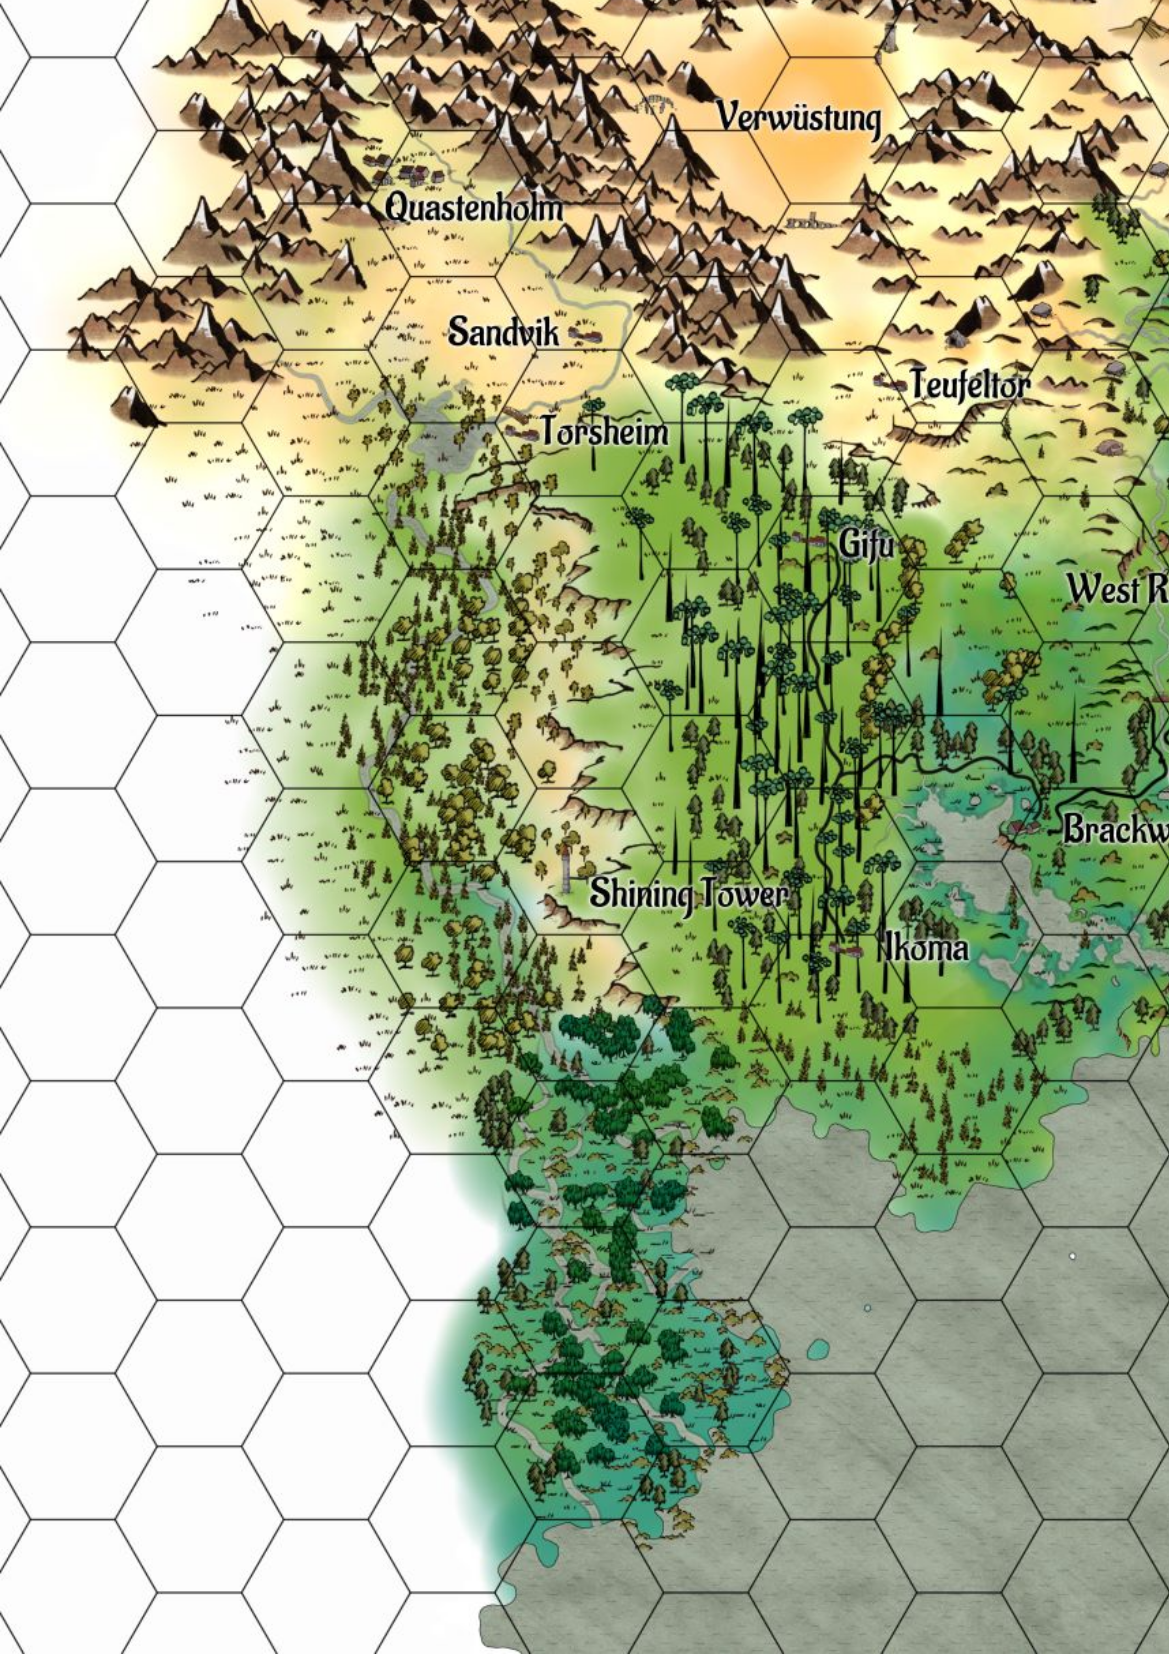
\includepdf{Backcover.pdf}
\end{document}
